\documentclass{article}
\usepackage[utf8]{inputenc}
\usepackage{enumitem}
\usepackage{dsfont}
\usepackage{amsmath}
\usepackage{graphicx}
\usepackage[colorlinks]{hyperref}
\usepackage{float}


\title{CS747 Assignemnt \#1}
\author{Hanish Dhanwalkar}
\date{\today}

\begin{document}

\maketitle

\section*{TASK 1}

\section{Explaination of code}
    \subsection{Upper Confidence Bound (UCB) Algorithm}
    \begin{enumerate}
        \item \textbf{Initialization:} \begin{itemize}
            \item Keeps track of the number of times each arm is pulled (counts) and the estimated value (values) of each arm.
            \item t keeps track of the total number of pulls.
        \end{itemize}

        \item \textbf{Arm Selection: \(give\_pull\):} \begin{itemize}
            \item For each arm, calculate the upper confidence bound (UCB) for that arm. Using \\ $UCB(i) = R_m + sqrt(\frac{2\times \log(t)}{n})$, where $R_m$ is mean reward, n= times arm i was pulled.
            \item The arm with the highest UCB value is selected.
        \end{itemize}


        \item \textbf{Updating Rewards \(get\_reward\):} \begin{itemize}
            \item Updates the mean reward estimate for the selected arm using an incremental formula: \\ $Q_n = \frac{(n-1)Q_{n-1}+R_n}{n}$, where $Q =$ value of the arm.
        \end{itemize}

        \item Regret vs. Horizon in \autoref{fig:ucb}.\ (plot generated by simulator.py)
    \end{enumerate}

    \subsection{KL-UCB Algorithm}
    \begin{enumerate}
        \item \textbf{Initialization:} \begin{itemize}
            \item Similar to UCB but uses KL divergence instead of a direct confidence bound.
            \item Keeps track of counts and values (mean rewards).
            \item $\epsilon$ (epsilon) is used as a precision threshold for numerical root-finding.
        \end{itemize}

        \item \textbf{Arm Selection: \(give\_pull\):} \begin{itemize}
            \item Uses Kullback-Leibler (KL) divergence to compute the upper confidence bound.
            \item Defines a function that measures how much the estimated mean p deviates from an optimistic bound q.
            \item Uses the bisection method to find q such that: \\ $KL(p,q) = \frac{\ln{t} + 3 \ln{\ln{t}}}{u_t}$, where $u_t$ is the number of times the arm has been pulled.
        \end{itemize}


        \item \textbf{Updating Rewards \(get\_reward\):} \begin{itemize}
            \item Updates the running mean estimate of the selected arm in the same way as UCB.
        \end{itemize}

        \item Regret vs. Horizon in \autoref{fig:kl_ucb}.\ (plot generated by simulator.py)
    \end{enumerate}

    \subsection{Thompson Sampling}
    \begin{enumerate}
        \item \textbf{Initialization:} \begin{itemize}
            \item Uses Beta distributions to model uncertainty in each arm’s reward probability.
            \item initiates $\alpha$ (successes) and $\beta$ (failures) for each arm, both initialized to 1.
        \end{itemize}

        \item \textbf{Arm Selection: \(give\_pull\):} \begin{itemize}
            \item Samples a random value from each arm’s $Beta(\alpha, \beta)$ distribution.
            \item The arm with the highest sampled value is selected.
        \end{itemize}


        \item \textbf{Updating Rewards \(get\_reward\):} \begin{itemize}
            \item If the selected arm gives a reward of 1, its $\alpha$ value is increased.
            \item If the reward is 0, its $\beta$ value is increased.
        \end{itemize}

        \item Regret vs. Horizon in \autoref{fig:thompson sampling}.\ (plot generated by simulator.py)
    \end{enumerate}

\newpage
\section{Results}
\begin{figure*}[hb]
    \centering
    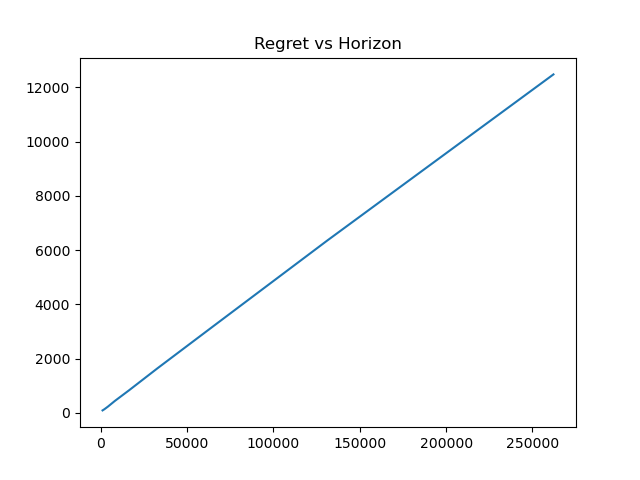
\includegraphics[width=0.68\linewidth]{../imgs/task1-Eps_Greedy-20250218-154744.png}
    \caption{Eps Greedy Algorithm. Regret vs. Horizon}\label{fig:eps_greedy}
\end{figure*}
\begin{figure*}[hb]
    \centering
    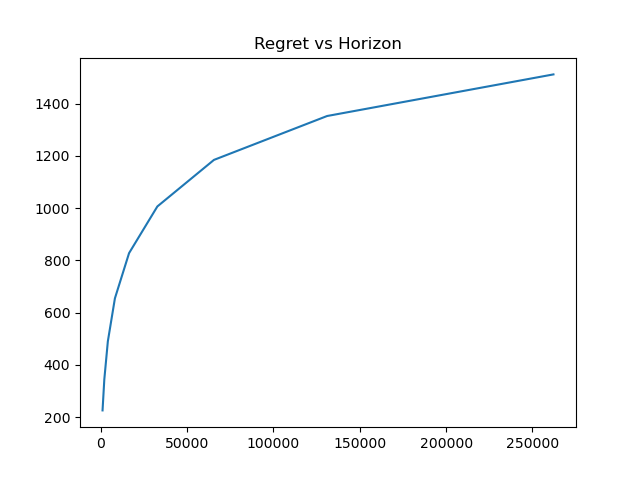
\includegraphics[width=0.68\linewidth]{../imgs/task1-UCB-20250218-155212.png}
    \caption{UCB Algorithm. Regret vs. Horizon}\label{fig:ucb}
\end{figure*}
\newpage
\begin{figure*}[hb]
    \centering
    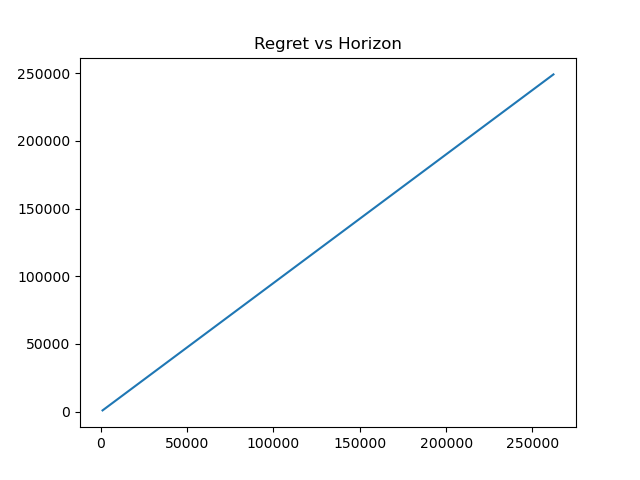
\includegraphics[width=0.68\linewidth]{../imgs/task1-KL_UCB-20250218-164050.png}
    \caption{KL-UCB Algorithm. Regret vs. Horizon}\label{fig:kl_ucb}
\end{figure*}
\begin{figure*}[hb]
    \centering
    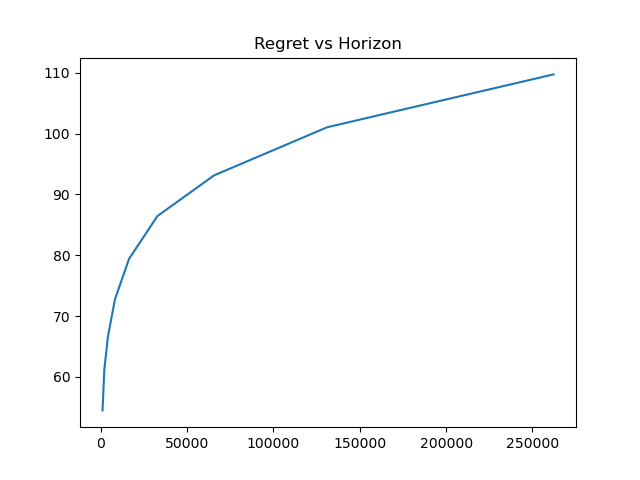
\includegraphics[width=0.68\linewidth]{../imgs/task1-Thompson_Sampling-20250218-164801.png}
    \caption{Thompson Sampling Algorithm. Regret vs. Horizon}\label{fig:thompson sampling}
\end{figure*}


\newpage
\section*{TASK 2}
\subsection{Approach}

    \begin{enumerate}
        \item \textbf{Tracking Rewards and Pulls:} \begin{itemize}
            \item Maintains 2 arrays \begin{itemize}
                \item $sum\_rewards$: Keeps track of the total rewards obtained for each arm.
                \item pulls: Stores how many times each arm has been pulled.
            \end{itemize}
            \item maintains a time step counter t to adjust confidence estimates over time.
        \end{itemize}

        \item \textbf{Upper Confidence Bound (UCB) Estimation:} \begin{itemize}
            \item Each arm’s expected value is estimated using UCB, which balances exploration and exploitation:
            \begin{equation}
                UCB(i) = R_m + sqrt(\frac{2\times \log(t)}{n})
            \end{equation}
            \item If an arm has never been pulled, it is given a high UCB value (1e5) to encourage initial exploration.
        \end{itemize}

        \item \textbf{Choosing the Query Set:} \begin{itemize}
            \item The arms are sorted in descending order of UCB values.
            \item evaluates different possible sizes (m) for the query set and selects the one that maximizes the expected net reward: 
            \begin{equation}
                \frac{\sum{UCB\ values\ of\ chosen\ arm -1}}{m}
            \end{equation}
        \end{itemize}

        \item When the oracle returns a pulled arm and its reward, the algorithm updates the reward and pull count for that specific arm.
    \end{enumerate}

\subsection{Explaination of the approach}
\begin{enumerate}
    \item The UCB-based selection ensures that the algorithm prioritizes arms that are promising while still exploring less-tested ones.
    \item By choosing the query set dynamically, it optimizes the trade-off between expected reward and cost.
    \item It avoids unnecessarily large query sets while still gaining useful information.

\end{enumerate}

\newpage
\section*{TASK 3}
Observations: 
\begin{enumerate}
    \item \textbf{Zero Epsilon:} When epsilon is very zero, algorithm predominantly exploits the best-known action. This can lead to lowest regret as no exploration is done and always pulls optimal arm here.
    \item \textbf{Medium Epsilon $0 < \epsilon < 1$:} When epsilon is between zero and one, the algorithm explores more frequently but also explores suboptimal actions, leading to higher regret.
    \item \textbf{1 Epsilon:} When epsilon is high, the algorithm explores more frequently but also explores suboptimal actions, leading to higher regret.
\end{enumerate}

\subsection*{Result:}

\begin{figure*}[hb]
    \centering
    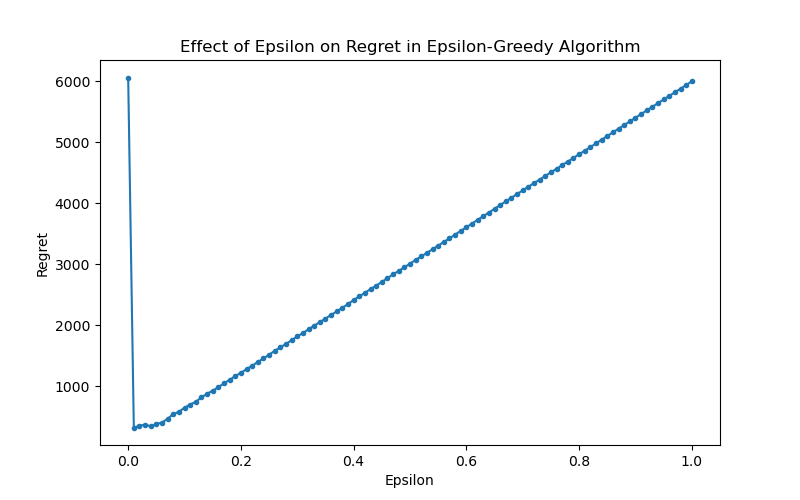
\includegraphics[width=0.68\linewidth]{../imgs/task3_regret_vs_epsilon.png}
    \caption{Eps Greedy Algorithm. Regret vs. Horizon}\label{fig:eps_greedy}
\end{figure*}


\end{document}
